\documentclass[conference]{IEEEtran}

\usepackage[latin1]{inputenc}	% for Latin languages
\usepackage[T1]{fontenc}	% for ISO and UTF characters
\usepackage[english]{babel}	% for multilingual support
\usepackage{graphicx}
\usepackage{subfig}

\newcommand{\fig}[4][htbp]{
  \begin{figure}[#1] {\centering\scalebox{#2}{\includegraphics{fig/#3}}\par}
    \caption{#4\label{#3}}
  \end{figure}
}

\newcommand{\epos}{\textsc{Epos}}

\begin{document}

\title{C-MAC: a Configurable Medium Access Control Protocol for Sensor Networks}

\author{Rodrigo Vieira Steiner, Tiago Rog�rio M�ck, and Ant�nio Augusto Fr�hlich \\
  \\
  Software/Hardware Integration Lab\\
  Federal University of Santa Catarina\\
  PO Box 476, 88040-900 - Florian�polis, SC, Brazil \\
  \{rodrigo,tiago,guto\}@lisha.ufsc.br
}

\maketitle

\begin{abstract}
C-MAC is a highly configurable MAC protocol realized as an
architecture of medium access control strategies that can be combined to produce
application-specific protocols. By selecting the proper strategies and
configuring their parameters, programmers can instantiate MAC protocols that
closely match their applications' requirements. C-MAC relies on static
metaprogramming techniques to achieve high configurability without compromising
size and performance. A previous implementation of C-MAC for the Mica2
mote produced B-MAC-like instances that are smaller, faster, and make better use
of the network than the original \textsc{TinyOS} B-MAC. In this work, we implemented 
and evaluated EPOS C-MAC in the scope of the EPOSMote project. The
EPOSMote devices used in this work feature an IEEE 802.15.4 compliant radio. This
motivated us to evaluate additional configuration parameters, including
synchronization (e.g. beacon-based), contention, and data handling (e.g. error
detection). As a result, C-MAC has undergone a major redesign and now features an
architecture whose elements are more fine-grained and thus can be reused in a larger
variety of scenarios.
% reescrever est� �ltima frase (ou as duas �ltimas)
\end{abstract}

\section{Introduction}
\label{sec:intro}
Wireless sensor networks~(WSN) are highly dependent on efficient Medium Access
Control~(MAC) protocols to make effective use of the few resources available on
traditional motes, bandwidth and energy in particular, but also memory and
processing power. This assertion is confirmed by the large number of MAC protocol
proposals available from the literature~\cite{bachir:2010}.

Nevertheless, most of the optimizations proposed by existing MAC protocols focus on
specific segments of the design space. What is considered an optimization by one
class of applications can represent a strong limitation for others. For instance,
a protocol optimized for massive data dissemination during a firmware update
operation (i.e. short, reliable, low-latency multicast) is certainly not the best
choice for sporadic environment monitoring (i.e. long-lasting, sporadic
unicasts). A MAC protocol aiming at covering a large fraction of the application
universe for sensor networks must feature configuration or adaptation mechanisms
directly controlled by applications. Fully automated decision making at system
level will never be able to match the knowledge programmers have about their
applications.

C-MAC is a highly configurable MAC protocol for WSN realized as an architecture of
medium access control strategies that can be combined to produce
application-specific protocols~\cite{wanner:2007}. It enables application
programmers to configure several communication parameters (e.g.  synchronization,
contention, error detection, acknowledgment, packing, etc) to adjust the protocol
to the specific needs of their applications. Although highly configurable, C-MAC
instances configured to mimic B-MAC produced better instances than the original
implementation in terms of footprint, performance, and network usage efficiency.
This is due to the static metaprogramming techniques used for the
implementation of C-MAC in C++, which enable aggressive compiler optimizations.

Nonetheless, the original C-MAC~\cite{wanner:2007} used configurable protocol elements that were
relatively coarse-grained. For instance, synchronization was taken as a single
large component that had to be reimplemented for any new protocol, even if aspects
such as preamble generation and timer synchronization are common to
virtually any protocol. The redesign presented here aimed at making C-MAC more
fine-grained, thus enabling the reuse of microcomponents in a larger variety of
application-specific protocols. The starting point for this new design was a
decomposition of traditional protocols of the three major categories~\cite{klues:2007}: channel
polling, scheduled contention, and time division multiple access.

Section~\ref{sec:cmac} describes the redesign of C-MAC in details. Section~\ref{sec:emote}
briefly describes the EPOSMote project, within which
this research was carried out. Section~\ref{sec:results} presents an
evaluation of the new C-MAC, and Section~\ref{sec:conclusions} concludes the paper.

\section{New C-MAC Design}
\label{sec:cmac}
A careful analysis of channel polling (e.g B-MAC~\cite{polastre:2004}, X-MAC~\cite{buettner:2006});
scheduled contention (e.g. S-MAC~\cite{ye:2002}, T-MAC~\cite{vandam:2003}); and TDMA protocols led us to the
new C-MAC architecture presented in Figures~\ref{cmac_act_sync},~\ref{cmac_act_receive}
and~\ref{cmac_act_send}. We used activity diagrams where each activity is executed by a microcomponent
which can have different implementations. These microcomponents alongside with the flow control
can be combined to produce application-specific protocols. By using static
metaprogramming techniques, microcomponents representing activities that do not make sense
for a certain protocol can be completely removed. When an activity is removed, its inputs 
are forwarded to the activity targeted by its outputs, still maintaining the original flow semantics.
Besides being able to accommodate representative protocols in any of the
three categories, C-MAC architecture also supports hybrid protocols such as Z-MAC and IEEE 802.15.4.

\fig{.3}{cmac_act_sync}{Synchronization Activity Diagram.}
\fig{.3}{cmac_act_receive}{Reception Activity Diagram.}
\fig{.3}{cmac_act_send}{Transmission Activity Diagram.}

C-MAC can be triggered either by send/receive events (i.e. when 
the target protocol has a full duty cycle) or periodically by time events 
(i.e. when a sleep/active duty cycle is required). The protocol remains \texttt{OFF},
with the radio turned off, until one of the previous events activates it. Figure~\ref{cmac_act_sync} 
presents the activities used to synchronize duty cycle. A node can start the synchronization by 
broadcasting~(\texttt{BROADCAST SYNC PKT}) a synchronization packet containing synchronization 
information (e.g. its schedule in a scheduled contention protocol) which is then followed by the 
reception of other nodes information~(\texttt{RX SYNC PKT}) like time slots allocation requests in 
a TDMA-based protocol. At this point, a node can either end its synchronization or perform additional
information exchange~(\texttt{TX SYNC PKT, RX SYNC RESP}) with the possibility of using a 
contention mechanism to avoid collisions in this process~(\texttt{CCA}). Note that in the same 
protocol each activity can be enabled, disabled, or perform different operations depending on the
node configuration (e.g. the node can be the master, slave, or both in a TDMA-based protocol).
After the node has been properly synchronized, it executes any transmission/reception request pending, otherwise it goes
\texttt{OFF} at the end of its active cycle. When the nodes are ready to transmit or receive, they may go through contention mechanisms 
in order to avoid collisions. These contention mechanisms are defined by the carrier sense~(\texttt{CCA}), and RTS/CTS~(\texttt{RX RTS, TX RTS, RX CTS, TX CTS}) microcomponents.

Some protocols do not require nodes to have a synchronized duty cycle, and thus does not exchange
synchronization data in order to communicate (e.g. B-MAC, X-MAC). This is done through the
transmission of a large preamble, or a sequence of short preambles~(\texttt{TX SYNC PREAMBLE,
RX SYNC PREAMBLE, RX ACK PREAMBLE, TX ACK PREAMBLE}).

After going through the contention mechanisms the nodes are ready to transmit or receive data. 
When the data is received~(\texttt{RX DATA}), it goes through the error handling and 
security mechanism~(\texttt{UNPACK}) and an acknowledgement packet can be transmitted~(\texttt{ACK TX}).
On the transmission side, error handling and security are appended to the data on 
the~\texttt{PACK} microcomponent before transmission~(\texttt{TX DATA}). The~\texttt{ACK RX} microcomponent implements 
acknowledgement packets reception. Some protocols allows the transmission of bursts of data packets (e.g. X-MAC and S-MAC)
without contending for the medium again, which required the \texttt{Keep alive} flows.

Through these new activity diagrams we were able to expand C-MAC and provide a larger range of
configurable points, while achieving a higher level of reuse. The main C-MAC configuration points now include:

\textbf{Physical layer configuration:} These are the configuration points defined
by the underlying transceiver (e.g. frequency, transmit power, date rate).

\textbf{Synchronization and organization:} Provides mechanisms to send or receive
synchronization data to organize the network and synchronize the nodes duty
cycle.

\textbf{Collision-avoidance mechanism:} Defines the contention mechanisms used to
avoid collisions. May be comprised of a carrier sense algorithm (e.g. CSMA-CA),
the exchange of contention packets (\emph{Request to Send} and \emph{Clear to
Send}), or a combination of both.

\textbf{Acknowledgment mechanism:} The exchange of \emph{ack} packets to
determine if the transmission was successful, including preamble acknowledgements.

\textbf{Error handling and security:} Determine which mechanisms will be used to
ensure the consistency of data (e.g. CRC check) and the data security.

\section{The EPOSMote}
\label{sec:emote}

The goal of the EPOSMote project is to develop an \epos-based WSN node focused on 
environmental monitoring~\cite{eposProject}. The nodes have the following main requirements:
\textbf{low energy consumption} (usually it is not practicable to often send teams
to the field to replace the nodes batteries, or the nodes may become inaccessible for
long time periods), \textbf{environmental monitoring features}(sensors to measure
environmental conditions), and \textbf{environmental integration}(the environment should not be affected by the
nodes presence and vice-versa, so the nodes must be as small, salubrious, and strong as possible).

Figure \ref{eposmote_block_diagram} shows an overview of the EPOSMote architecture.
Its hardware is designed as a layer architecture composed by a main module,
a sensoring module, and a power module. The main module is responsible for processing
and communication. It is based on the ATmega1281~\cite{atmel:ATMEGA1281} microcontroller 
and the AT86RF230~\cite{atmel:AT86RF230} radio from Atmel. We have developed a sensoring module 
based on the SHT11 sensor, which is used to measure the environment temperature and humidity. 
Yet expensive, we chose this sensor due to its very small size. Figure \ref{eposmote_pound_bw}
shows the final hardware. The EPOSMote is littler than a �2 coin.

%\fig{.35}{eposmote_block_diagram}{Architectural overview of EPOSMote.}

%\fig{.08}{eposmote_pound}{EPOSMote side-by-side with a �2 coin.}

%\begin{figure}
%  \centering
%  \subfloat[]{\label{eposmote_block_diagram}\scalebox{0.37}{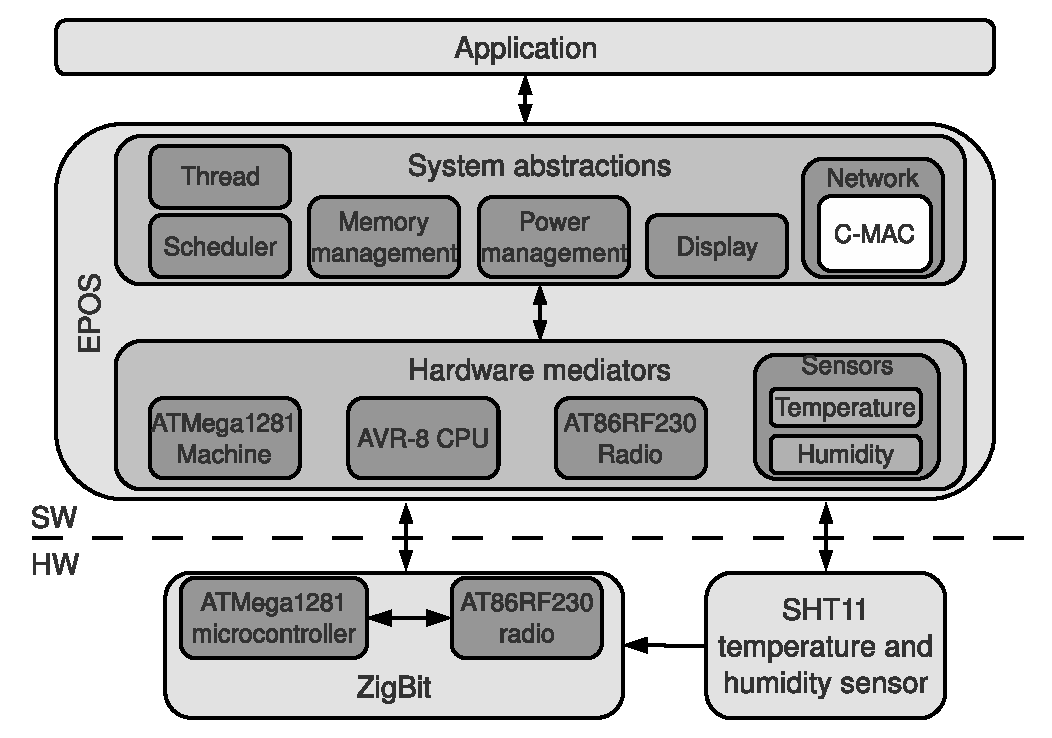
\includegraphics{fig/eposmote_block_diagram}}} \\
%  \subfloat[]{\label{eposmote_pound_bw}\scalebox{0.13}{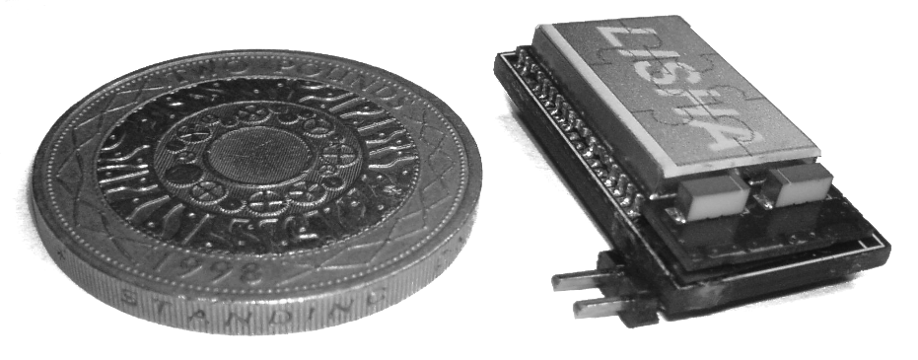
\includegraphics{fig/eposmote_pound_bw}}}
%  \caption{Architectural overview of EPOSMote (a) EPOSMote side-by-side with a �2 coin (b).}
%  \label{fig_arch_test_all}
%\end{figure}
 \begin{figure}[ht]
 \begin{minipage}{0.37\linewidth}
   \centering
   \subfloat[]{\label{eposmote_block_diagram}\scalebox{0.37}{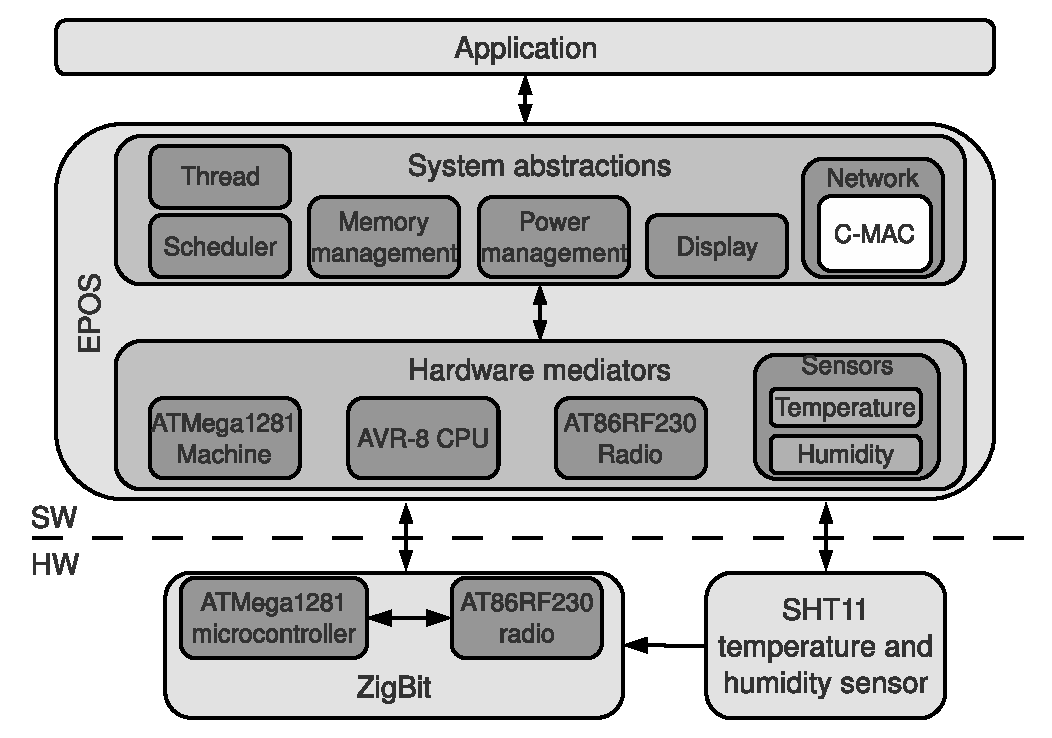
\includegraphics{fig/eposmote_block_diagram}}} \\
 \end{minipage}
 %\hspace{0.5cm}
\hspace{0.35\linewidth}
 \begin{minipage}{0.13\linewidth}
   \centering
   \subfloat[]{\label{eposmote_pound_bw}\scalebox{0.13}{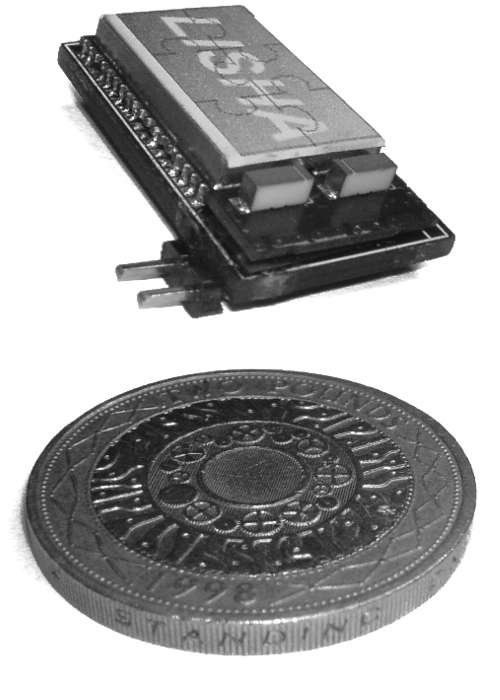
\includegraphics{fig/eposmote_pound_bw2}}}
 \end{minipage}
\caption{(a) Architectural overview of EPOSMote. (b) EPOSMote side-by-side with a �2 coin.}
  \label{fig_arch_test_all}
\end{figure}


\section{Experimental results}
\label{sec:results}

In order to evaluate C-MAC we have implemented a configurable IEEE 802.15.4 MAC on the EPOSMote.
C-MAC was configured to bahave like following MACs, which were based on IEEE 802.15.4: 
\textbf{Beacon-enabled IEEE 802.15.4}; \textbf{Non-beacon IEEE 802.15.4}; 
\textbf{Non-beacon IEEE 802.15.4 without CSMA-CA}; \textbf{Non-beacon IEEE 802.15.4 without ACK}; 
and \textbf{Non-beacon IEEE 802.15.4 without both CSMA-CA and ACK}.

In the experimets, we have used an network topology that simulates a typical monitoring application,
where an coordinator receives data transmitted periodically by other nodes monitoring the environment.
One node is defined as the coordinator and other nodes are placed around the coordinator. The nodes
are placed in a way in which they are within range of each other, so each node may potentially interfere
in the communications of every other node. For all experimets we used: GCC 4.0.2 to compile EPOS and 
the application; the ATMEGA1281 clock set to 1 MHz; packets size of 64 bytes; 3 dBm of TX power; for 
the beacon-enabled configurations, beacon and superframe order ware set to 7 and 4, yielding a 
duty cycle of 12 \%.

%\fig{.5}{results_net_topology}{Network topology used on the evaluation.}

%\begin{table}[h]
%\caption{Configuration parameters used on the experiments}
%\label{results_table_params}
%\centering
%\begin{tabular}{ll}
%\hline\noalign{\smallskip}
%Parameter & Value \\
%\noalign{\smallskip}
%\hline
%\noalign{\smallskip}
%Compiler & GCC 4.0.2 \\
%Microcontroller clock & 1 MHz \\
%Packet size & 64 bytes \\
%TX power & 3 dBm \\
%Beacon order & 7 \\ 
%Superframe order & 4 \\ 
%Duty cycle & 12\% \\ 
%\hline
%\end{tabular}
%\end{table}

\subsection{Results}

We have used the avr-size tool, from GNU Binutils version 2.19, to analyse the size of the applications. 
The result for each configuration is shown in Table \ref{results_table}. As expected, 
the more complex the configuration, the larger the footprint. Thus, the configuration with no beacons,
CSMA, and ACK yielded the smallest footprint, while the full IEEE 802.15.4 configuration yielded the 
largest one. Also, we compared C-MAC with the IEEE 802.15.4 MAC provided by Meshnetics 
ZigBeeNet~\cite{ZigBeeNet} for the ATMega1281/AT86RF230. C-MAC's meta-programmed implementation, 
along with EPOS's component architecture, delivered equivalent functionality with smaller footprint than
a non-configurable, platform-optimized implementation.


% As for the data area, which is equal for all configurations, this is due to a implementation issue, but it can be even improved, which is already in our future work list.
%In order to evaluate the memory used by local variable, consider measuring the max stack size or something like that

%\fig{.6}{results_plot_mem}{Memory footprint}
\begin{table}[h]
\caption{Memory footprint and latency of C-MAC IEEE 802.15.4 and ZigBeeNet IEEE 802.15.4. The latency is the round-trip time between two nodes.}
\label{results_table}
\centering
\scriptsize
\begin{tabular}{lccc}
\hline\noalign{\smallskip}
Configuration & Code (bytes) & Data (bytes) & RTT (ms)\\
\noalign{\smallskip}
\hline
\noalign{\smallskip}
No CSMA-CA / ACK & 3248 & 185 & 60 \\
No ACK & 3572 & 185 & 68 \\ 
No CSMA-CA & 3768 & 202 & 71 \\ 
CSMA-CA / ACK enabled & 4092 & 202 & 79 \\ 
CSMA-CA / ACK  beacons enabled & 5344 & 215 & 1882 \\
ZigBeeNet MAC (non-beacon) & 26776 & 289 & 62 \\
\hline
\end{tabular}
\end{table}

To evaluate latency, we have measured the round-trip time of a packet between two nodes. 
The results in Table \ref{results_table} show that the latency increases as more features
of the protocol are enabled. On a beacon enabled network, duty cycle of 12\% results in a sleep 
period of about 2 seconds, which is the dominating factor when this configuration is used. However, 
the time spent with idle listening is reduced, thus reducing the energy consumption as shown in 
Figure~\ref{results_plot_energy}. Also, C-MAC latency is comparable the ZigBeeNet MAC, which shows 
that C-MAC configurability does not come at expense of performance.

%\fig{.6}{results_plot_latency}{Latency}


Figure \ref{results_plot_throu} shows the variations of the average throughput as the number of nodes
on the network increases. The overall throughput improves as the features of the protocol are removed 
and presents small variations as the number of nodes increase, this is due to the low network traffic 
and the non-coincidence of the period of transmission of the nodes. The exception is when we enable the 
use of ACK packets and disable CSMA-CA. With this configuration there is a high packet loss due to collisions
and the retransmissions ends up reducing the protocol's performance. 

\fig{.4}{results_plot_throu}{Average network throughput (logarithmic scale).}

The low duty cycle used on the \emph{CSMA-CA / ACK  beacons enabled} configuration yielded the worse throughput.
This configuration also yielded the biggest performance deterioration with the increase in the number of nodes.
This is due to the fact that all nodes try to communicate at the same small period, increasing the chance of 
collisions and packet loss rate, as shown in Figure \ref{results_plot_pkt_loss}. For configurations without beacon
synchronization, the packet loss rate varies similar to the throughput.

\fig{.4}{results_plot_pkt_loss}{Average packet loss rate.}

C-MAC's energy efficiency were evaluated by measuring the energy consumed per byte received at the coordinator. 
Figure \ref{results_plot_energy} shows the results. As expected, the configurations with beacon synchronization
yielded the best results. Except for the beacon-enabled configuration, the energy per byte decreases as the number
of nodes increases. This happens because the main source of energy consumption is idle listening. As the network
traffic increases, the average energy consumed per byte decreases. This is not the case on the beacon-enabled configuration,
showing that it successfully treated the idle listening problem.

\fig{.4}{results_plot_energy}{Energy consumed per byte received on the coordinator.}

%\subsection{Discussion}
%
%With C-MAC, it is possible to configure the protocol according to the application's requirements. The results 
%showed that we can easily control the trade-offs among memory footprint, latency, throughput, 
%reliability and energy consumption, by using different configurations of IEEE 802.15.4. For example, 
%on environments which there are a big number of nodes transmitting very often, but there is no need 
%to guarantee the delivery of messages, an implementation without acknowledgment packets can be used to 
%increase the network throughput. On environments that contains a big number of nodes that transmit as little 
%as possible to save energy, a configuration with CSMA-CA and acknowledgment packets can be used to guarantee the 
%message exchange. On applications with more tolerant energy consumption requirements, the beacons can be disabled to
%obtain higher throughput and lower latency.
%
%Table~\ref{results_table} shows the memory footprint and latency of the IEEE 802.15.4 MAC 
%provided by Meshnetics ZigBeeNet~\cite{ZigBeeNet} for the ATMega1281/AT86RF230, along with the results obtained from 
%the C-MAC evaluation.  C-MAC achieved smaller memory footprint, and performance comparable to a non-configurable, 
%platform-optimized implementation. This shows that C-MAC configurability does not come at expense of performance or 
%code size.

\section{Conclusion}
\label{sec:conclusions}
This paper presented the new design of C-MAC, a highly configurable, low-overhead
Medium Access Control protocol for Wireless Sensor Networks. This new design was
developed within EPOSMote, a project targeted at enabling application-specific
deployment scenarios for IEEE 802.15.4 networks. The new C-MAC arose from a
careful decomposition of several preexisting MAC protocols aiming at obtaining
their state machines. These individual state machines were subsequently merged
into a generalized one and captured as a component architecture that can be
specialized to produce a large variety of application-specific protocols. The
architecture was implemented in C++ using static metaprogramming techniques (e.g.
templates, inline functions, and inline assembly), thus ensuring that
configurability does not come at expense of performance or code size. 

We experimentaly evaluated C-MAC in terms of memory footprint, latency,
throughput, packet loss rate, and energy consumption by varying IEEE 802.15.4
main configuration aspects. The results corroborate the new design with figures
comparable to the non-configurable, platform-optimized implementation provided by
Meshnetics. %%%%%% VERIFICAR!
Applications using EPOSMote can now easily configure a MAC
protocol to closely match their requirements.
   
\bibliographystyle{IEEEtran}
\bibliography{references.bib}

\end{document}
